\documentclass{article}
\usepackage[T1]{fontenc} % codificação da fonte em 8-bits
\usepackage[utf8]{inputenc} % acentuação direta
\usepackage[brazil]{babel} % em portugues brasileiro
\usepackage[normalem]{ulem}
\useunder{\uline}{\ul}{}
\usepackage{graphicx}
\usepackage[utf8]{inputenc}
\usepackage{fullpage}
\usepackage{listings}
\usepackage{xcolor}
\usepackage{amsmath}
\usepackage{amssymb}
\usepackage{url}
\usepackage{hyperref}
\usepackage[linesnumbered,ruled,vlined]{algorithm2e}
% \usepackage{enumitem}
\usepackage[shortlabels]{enumitem}
\usepackage{listings}
\lstset { %
    language=C++,
    backgroundcolor=\color{black!5}, % set backgroundcolor
    basicstyle=\footnotesize,% basic font setting
}

\definecolor{mygreen}{rgb}{0,0.6,0}

% set the default code style
\lstset{
    language=C++,
    frame=tb, % draw a frame at the top and bottom of the code block
    tabsize=4, % tab space width
    showstringspaces=false, % don't mark spaces in strings
    numbers=none, % display line numbers on the left
    commentstyle=\color{mygreen}, % comment color
    keywordstyle=\color{blue}, % keyword color
    stringstyle=\color{red}, % string color
    backgroundcolor=\color{black!5}, % set backgroundcolor
    basicstyle=\footnotesize,% basic font setting
    literate = {-}{-}1, % <------ trick for '-' in shell commands
}

\parindent0in
\pagestyle{plain}
\thispagestyle{plain}

\newcommand{\assignment}{Lista 5}
\newcommand{\duedate}{20 de maio}


\title{Lista 5}
\date{}

\begin{document}

Fundação Getulio Vargas\hfill\\
Estruturas de Dados\hfill\textbf{\assignment}\\
Prof.\ Jorge Poco\hfill\textbf{Entrega:} \duedate\\
\smallskip\hrule\bigskip

{\let\newpage\relax\maketitle}
\maketitle

\section{Questões Teóricas}

\paragraph{Problema 1.} (20 pontos)

Em árvores \textit{scapegoat}, mostramos que se \texttt{size(u.child)/size(u) $\leq \dfrac{2}{3}$} para cada nó de uma árvore, então a altura da árvore é no máximo $\log_{3/2} n$. Neste problema, vamos generalizar isso
condição para:

\begin{equation*}
    \dfrac{\texttt{size(u.child)}}{\texttt{size(u)}} \leq \alpha
\end{equation*}

para alguma constante $\alpha$.

\begin{itemize}
\item Por que não faz sentido definir $\alpha$ maior que 1 ou menor que $\dfrac{1}{2}$?
\item Se cada nó de uma árvore de $n$-nós satisfaz a condição acima, o que pode ser dito sobre a altura da árvore em função de $n$ e $\alpha$? Justifique brevemente sua resposta.
\end{itemize}

\paragraph{Resposta 1.}

\paragraph{Problema 2.} (15 pontos)

Qual é o objetivo de um ponteiro \textit{next-leaf} nas árvores B+?

\paragraph{Resposta 2.}

\paragraph{Problema 3.} (15 pontos) 
Afirmamos que as árvores \textit{scapegoat} são eficientes no sentido amortizado, mas operações \texttt{find} em árvores \textit{scapegoat} são eficientes mesmo no pior dos casos. Por que isso vale?

\paragraph{Resposta 3.}

\paragraph{Problema 4.} (20 pontos)

Considere as árvores B de ordem 4 mostradas na Fig.~\ref{fig:prob4} abaixo. Lembre-se de que cada não-folha
nó tem entre 2 e 4 filhos, e cada nó-folha tem entre 1 e 3 chaves. Vamos supor
duas convenções. Primeiro, a rotação das chaves (quando possível) tem precedência sobre a divisão/fusão (\textit{splitting}/\textit{merging}).
Segundo, ao dividir um nó, se o número de chaves compartilhadas pelos dois novos nós for ímpar
número, o nó mais à esquerda recebe o maior número de chaves.

\begin{figure}[h]
    \centering
    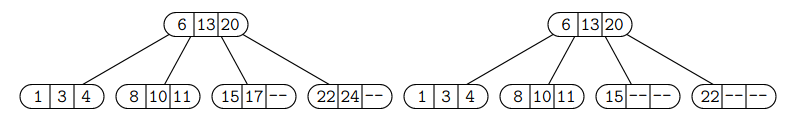
\includegraphics[width = 0.8\linewidth]{fig1.png}
    \caption{Operações com a árvore B.}
    \label{fig:prob4}
\end{figure}

\begin{itemize}
    \item (a) Mostre a árvore B resultante após inserir a chave 9 na árvore da Fig.~\ref{fig:prob4}(a).
\item (b) Mostre a árvore B que resulta depois de inserir a chave 2 na árvore (original) da Fig.~\ref{fig:prob4}(a).
\item (c) Mostre a árvore B que resulta após excluir a chave 22 da árvore da Fig.~\ref{fig:prob4}(b).
\end{itemize}

\paragraph{Resposta 4.}

\paragraph{Problema 5.} (15 pontos)

Tanto as \textit{skiplists} quanto as árvores B fizeram uso de nós contendo um número variável de elementos.
(Na \textit{skiplists}, um nó tem um número variável de ponteiros e em uma árvore B um nó
tem um número variável de chaves/filhos.) Em uma delas, alocamos nós de tamanho variável
e na outra alocamos nós de mesmo tamanho fixo. Esclareça qual estrutura tem nós de tamanho fixo e qual não tem, e explique porquê fazemos de maneira distintas nesses dois casos.

\paragraph{Resposta 5.}

\paragraph{Problema 6.} (15 pontos)

Tanto as árvores \textit{scapegoat} quanto as árvores de \textit{splay} fornecem tempo amortizado $O(\log n)$ para
operações de dicionário padrão (inserir, excluir e encontrar). Suponha que seu aplicativo
envolve muito mais operações de encontrar do que inserções ou exclusões. Qual desses dois
estruturas que você prefere e por que?

\paragraph{Respota 6}

\section{Detalhes avaliação}
Uma pergunta comum é "quanto detalhe é esperado nas respostas?", algumas orientações são:
%
\paragraph{Provar vs. Mostrar:}
Se lhe pedirmos para “provar” algo, estamos à procura de uma prova bem estruturada. Se você estiver aplicando a indução, tenha cuidado para distinguir seu(s) caso(s) básico(s) e indicar qual é a sua hipótese de indução. Se lhe pedirmos para “mostrar”, “explicar” ou “justificar”, estaremos geralmente apenas esperando uma explicação em português. Se você não tiver certeza, por favor, verifique.

\paragraph{Algoritmo vs. Pseudocódigo:} Quando pedimos um “algoritmo” estamos esperando uma descrição em alto nível de algum processo computacional, geralmente em uma combinação de português e notação matemática (por exemplo, “classifique as $n$ chaves e localize $x$ usando busca binária”). Para pseudocódigo, nós estão esperando uma descrição passo a passo mais detalhada que se pareça muito mais com C++ (por exemplo, “\texttt{Node q = p.left}”). Lembre-se de que você está escrevendo seu código para ser lido por um humano, e não por um compilador. Por favor, omita detalhes irrelevantes que são sintaxes de C++. Mesmo que não solicitemos explicitamente, sempre que você fornecer um algoritmo ou pseudocódigo, você deve sempre fornecer uma breve explicação em português. Isso ajuda o avaliador a entender quais são suas intenções, e se houver um pequeno erro em seu código, muitas vezes podemos usar seu explicação para entender quais eram suas reais intenções.

\end{document}
